% Model_2Db.tex
% TikZ recreation of the flat-sky lensing set-up figure (replaces Model_2Db.jpeg)
\documentclass[border=4pt]{standalone}
\usepackage{tikz}
\usepackage{amsmath}
\usetikzlibrary{arrows.meta, decorations.markings, calc}

\definecolor{axiscol}{RGB}{20,20,20}
\definecolor{planecol}{RGB}{150,150,150}
\definecolor{lenscol}{RGB}{224,145,45}
\definecolor{imgcol}{RGB}{235,205,60}
\definecolor{veccol}{RGB}{175,30,30}
\definecolor{anglecol}{RGB}{110,45,140}
\definecolor{obscol}{RGB}{60,120,200}

\begin{document}
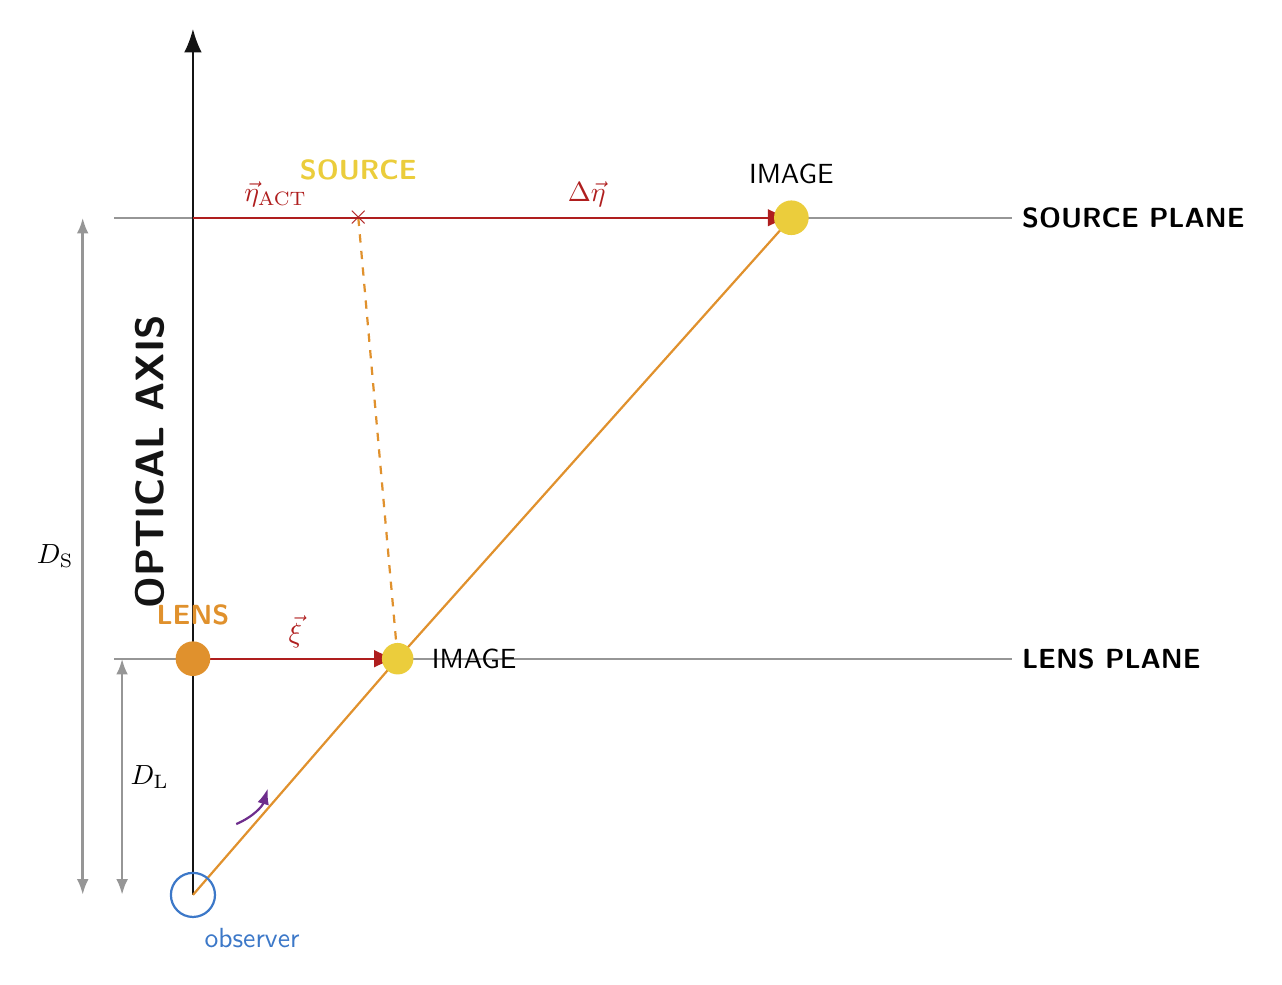
\begin{tikzpicture}[
    >=Latex,
    line width=1pt,
    font=\sffamily
  ]

  % --- coordinates -----------------------------------------------------
  \coordinate (Observer)    at (0,0);
  \coordinate (Lens)        at (0,3);
  \coordinate (LensImg)     at (2.6,3);
  \coordinate (Source)      at (2.1,8.6);
  \coordinate (SourceImg)   at (7.6,8.6);
  \coordinate (AxisTop)     at (0,11);

  % --- plane lines -------------------------------------------------------
  \draw[planecol, thick] (-1,3)   -- (10.4,3)   node[right, black, font=\sffamily\bfseries] {LENS PLANE};
  \draw[planecol, thick] (-1,8.6) -- (10.4,8.6) node[right, black, font=\sffamily\bfseries] {SOURCE PLANE};

  % --- optical axis --------------------------------------------------
  \draw[axiscol, thick, -{Latex[length=3mm]}] (Observer) -- (AxisTop);
  \node[axiscol, rotate=90, font=\sffamily\bfseries\Large] at (-0.55,5.5) {OPTICAL AXIS};

  % --- distance measures (D_S, D_L) -----------------------------------
  \draw[planecol, {Latex[length=2mm]}-{Latex[length=2mm]}] (-1.4,0) -- (-1.4,8.6);
  \node[black, font=\sffamily\bfseries] at (-1.75,4.3) {$D_{\mathrm S}$};

  \draw[planecol, {Latex[length=2mm]}-{Latex[length=2mm]}] (-0.9,0) -- (-0.9,3);
  \node[black, font=\sffamily\bfseries] at (-0.55,1.5) {$D_{\mathrm L}$};

  % --- light rays (bent at the lens plane) ----------------------------
  \draw[lenscol, thick] (Observer) -- (LensImg) -- (SourceImg);
  \draw[lenscol, thick, dashed] (Source) -- (LensImg);

  % deflection angle marker
  \draw[anglecol, thick, -{Latex[length=2mm]}]
    (0.55,0.9) to[bend right=25] (0.95,1.35);

  % --- vectors in the two planes --------------------------------------
  \draw[veccol, thick, -{Latex[length=3mm]}] (Lens) -- (LensImg)
    node[midway, above, font=\sffamily] {$\vec{\xi}$};

  \draw[veccol, thick, -{Latex[length=3mm]}] (0,8.6) -- (SourceImg);
  \node[veccol, font=\sffamily] at (1.05,8.9) {$\vec{\eta}_{\mathrm{ACT}}$};
  \node[veccol, font=\sffamily] at (5.0,8.9)  {$\Delta\vec{\eta}$};

  % --- lens, source, and image markers --------------------------------
  \fill[lenscol] (Lens) circle (0.22);
  \node[lenscol, font=\sffamily\bfseries, anchor=south] at ($(Lens)+(0,0.3)$) {LENS};

  \fill[imgcol] (LensImg) circle (0.2);
  \node[black, font=\sffamily, anchor=west] at ($(LensImg)+(0.3,0)$) {IMAGE};

  \fill[imgcol] (SourceImg) circle (0.22);
  \node[black, font=\sffamily, anchor=south] at ($(SourceImg)+(0,0.3)$) {IMAGE};

  \node[veccol, font=\sffamily] at (Source) {$\times$};
  \node[imgcol, font=\sffamily\bfseries, anchor=south] at ($(Source)+(0,0.35)$) {SOURCE};

  % --- observer icon ---------------------------------------------------
  \draw[obscol, thick] (Observer) circle (0.28);
  \node[obscol, font=\sffamily] at (0.75,-0.55) {observer};

\end{tikzpicture}
\end{document}
